\section{Assignment 4: Image Stitching}
\label{sec:assignment4}


\subsection{SIFT Interest Point Detection}

In the first step we use the SIFT algorithm for key point detection. As we do not need the key descriptors at this stage, we only acquire the position of each key point along with their scale and orientation. SIFT uses the Difference of Gaussians (DoG) to approximate LoG. To define different scales, the SIFT algorithm creates a minimum of five different Gaussian images per octave, the difference of these images (DoGs) are then used for Maxima detection, similar to blob detection algorithm. 

\begin{figure}[h]
	\centering
	\begin{tabular}{cc}
	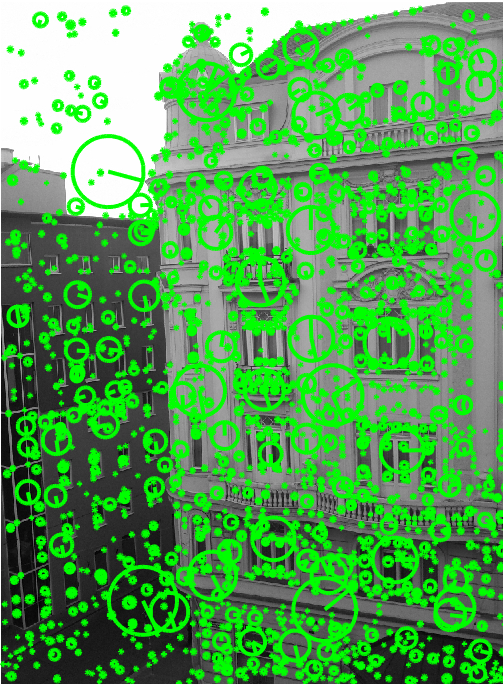
\includegraphics[width=0.48\textwidth]{figures/vl_plotframe_officeview1.png} &
	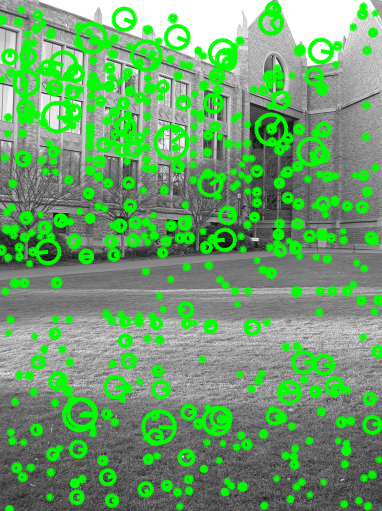
\includegraphics[width=0.48\textwidth]{figures/vl_plotframe_campus4.png} 

	\end{tabular}
	\caption{SIFT key point detection: scale and orientation of key points.}
	\label{fig:a4:vlplotframe}
\end{figure}

To find the orientation of the key points, depending on the scale, a region around the key point center is chosen. The magnitudes and orientations are calculated for each pixel in this region, and the result is placed in a histogram made of 36 bins (10degrees per bin). The highest point of the histogram is the orientation of the key point. Any other peak close to the highest point is converted into a new key point (same position and scale, but with a different orientation). The key point orientation is important, because further calculations (descriptors) will be relative to this orientation, which ensures orientation invariance for matching key points.

The function \texttt{vl\_plotframe} illustrates the results. The circle corresponds to the associated scale of the key point and the line is its orientation as visualized in Figure \ref{fig:a4:vlplotframe}.

\subsection{Interest Point Matching and Image Registration}

Similar to step A, first we extract all key points via SIFT, this time along with the associated descriptors of each key point. The descriptors are an array of 128 numbers constructed as follows: First the 16x16 window around the key point is broken down into smaller 4x4 windows. Within each of the 16 windows the gradients are calculated and subsequently put into an 8 bin histogram (45 degrees each). The magnitude added by each gradient also depends on the distance from the key point (using gaussian weights). 

Each of the 128 resulting numbers will be normalized and reduced by the key point's orientation (to ensure orientation invariance) and subsequently clamped at 0.2 (to ensure illumination invariance) before being normalized to unit vector again.

\begin{figure}[h]
	\centering
	\begin{tabular}{cc}
	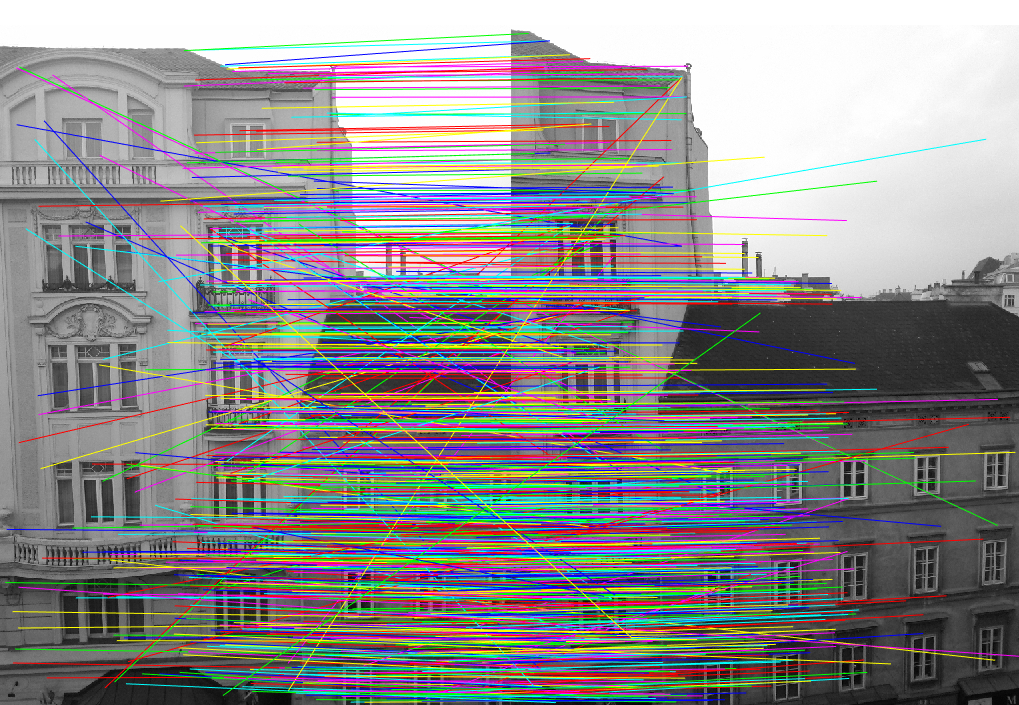
\includegraphics[width=0.75\textwidth]{figures/vl_ubcmatch1.png} \\
	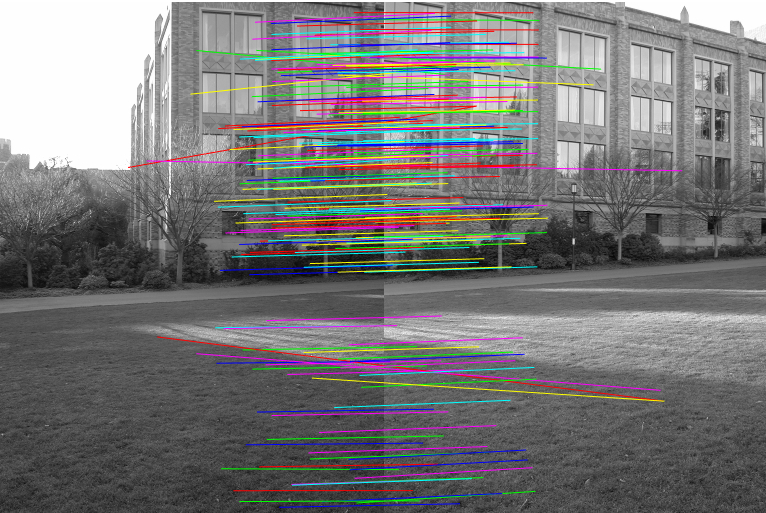
\includegraphics[width=0.75\textwidth]{figures/vl_ubcmatch2.png} 

	\end{tabular}
	\caption{The resuts of \texttt{vl\_ubcmatch}. }
	\label{fig:a4:ubcmatch}
\end{figure}

\texttt{vl\_ubcmatch} is used as a first, basic, matching step. For each descriptor in the first image, \texttt{vl\_ubcmatch} attempts to find the closest descriptor in the target image using L2 norm of the difference between the two. This basic algorithm may consequently return many false positive matches as well. The result is illustrated by Figure \ref{fig:a4:ubcmatch}.

To eliminate potential false positive matches, a RANSAC scheme is applied. Basically, we estimate the correct homography  by using 4 random sample matches out of all matches found by \texttt{vl\_ubcmatch} before applying them to all other key points via \texttt{transformPointsforward}. Subsequently we keep only those matches which are inliers, that is their euclidean distance is smaller than a certain threshold T. The RANSAC algorithm is applied N times and the homography  with the largest number of inliers is returned as the correct estimation. 

The result is presented in Figure \ref{fig:a4:ransac}.

\begin{figure}[h]
	\centering
	\begin{tabular}{cc}
	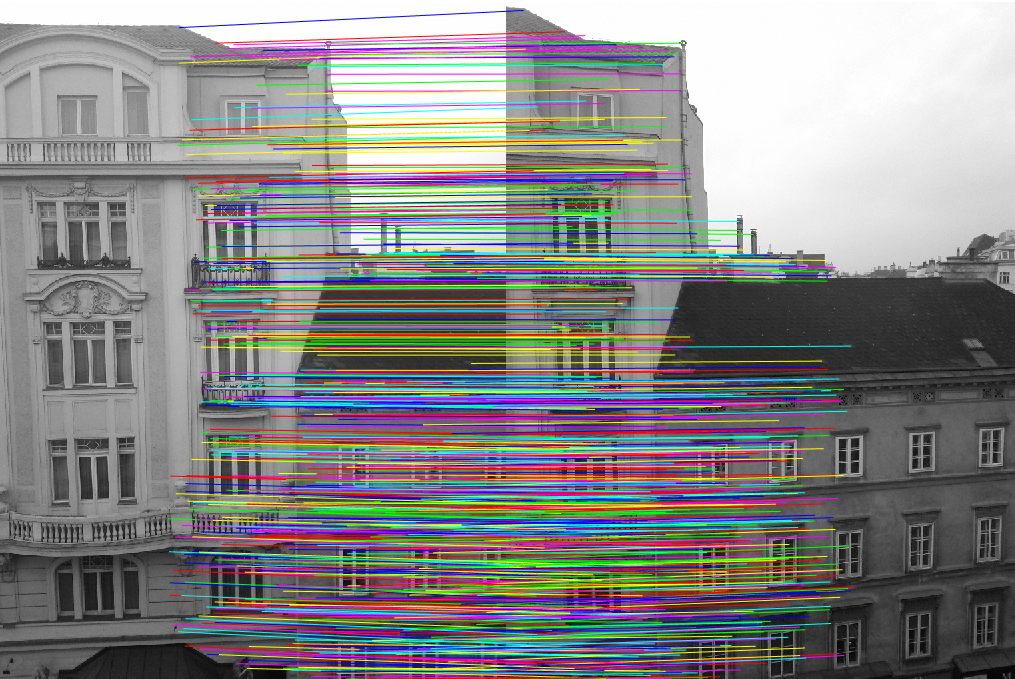
\includegraphics[width=0.8\textwidth]{figures/ransac1.png} \\
	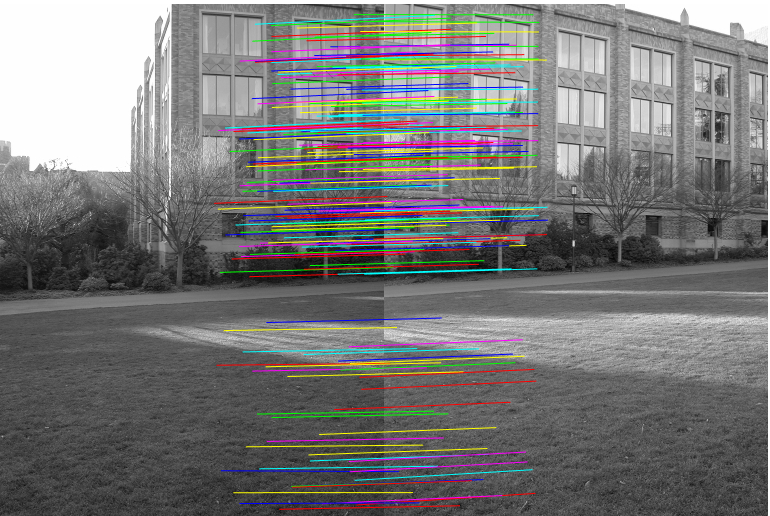
\includegraphics[width=0.8\textwidth]{figures/ransac2.png} 

	\end{tabular}
	\caption{The matched key points after applying RANSAC. }
	\label{fig:a4:ransac}
\end{figure}


Figure \ref{fig:a4:ransac_removes} illustrates the potential false positive matches that are eliminated after applying RANSAC.


\begin{figure}[h]
	\centering
	\begin{tabular}{cc}
	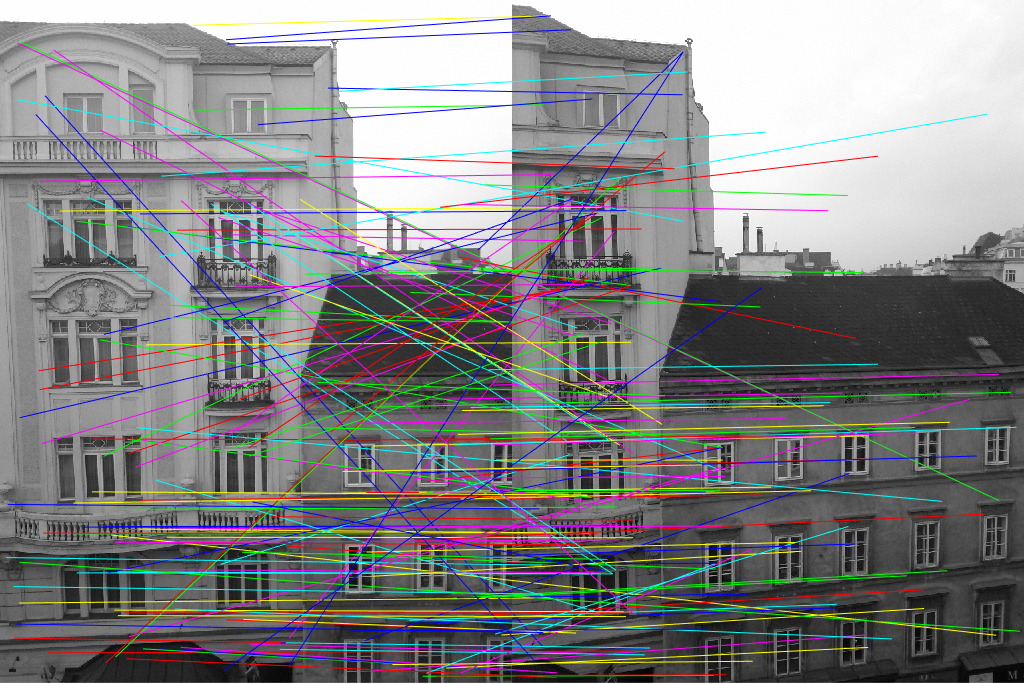
\includegraphics[width=0.45\textwidth]{figures/ransac_removes1.png} &
	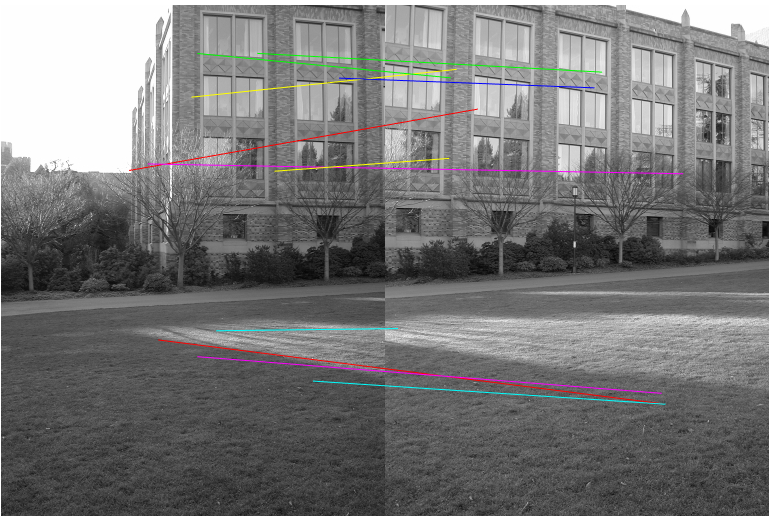
\includegraphics[width=0.45\textwidth]{figures/ransac_removes2.png} 

	\end{tabular}
	\caption{Potentially false positive matches estimated by \texttt{vl\_ubcmatch}. }
	\label{fig:a4:ransac_removes}
\end{figure}


\begin{figure}[h]
	\centering
	\begin{tabular}{cc}
	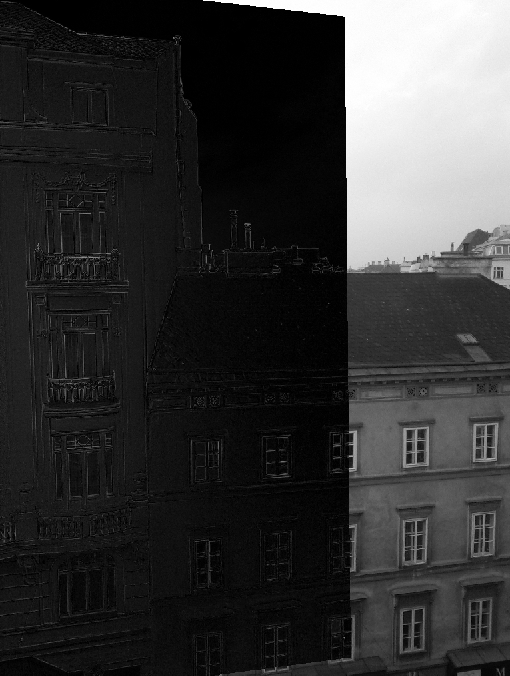
\includegraphics[width=0.23\textwidth]{figures/diff1.png} 
	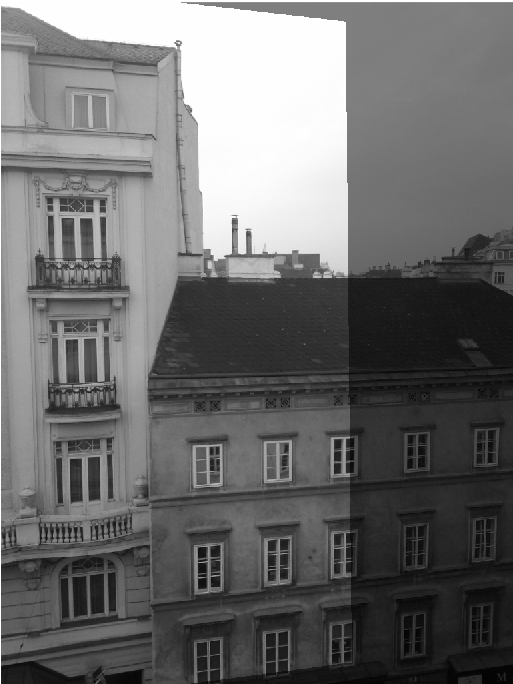
\includegraphics[width=0.23\textwidth]{figures/overlay1.png} 
	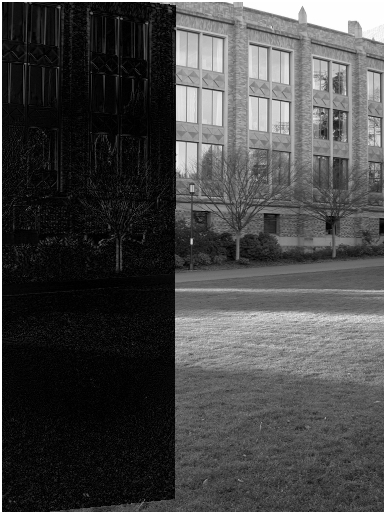
\includegraphics[width=0.23\textwidth]{figures/diff2.png} 
	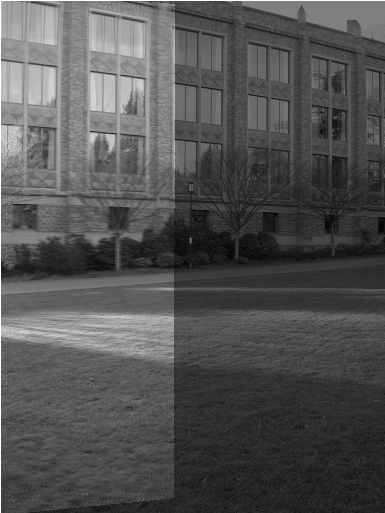
\includegraphics[width=0.23\textwidth]{figures/overlay2.png} 

	\end{tabular}
	\caption{Difference and overlay view of aligned images.}
	\label{fig:a4:diffs}
\end{figure}


After applying the above steps the images are already well aligned as presumed. Figure \ref{fig:a4:diffs} shows a collection of absolute differences of pairs of matched images. 



\begin{figure}[h]
	\centering
	\begin{tabular}{cc}
	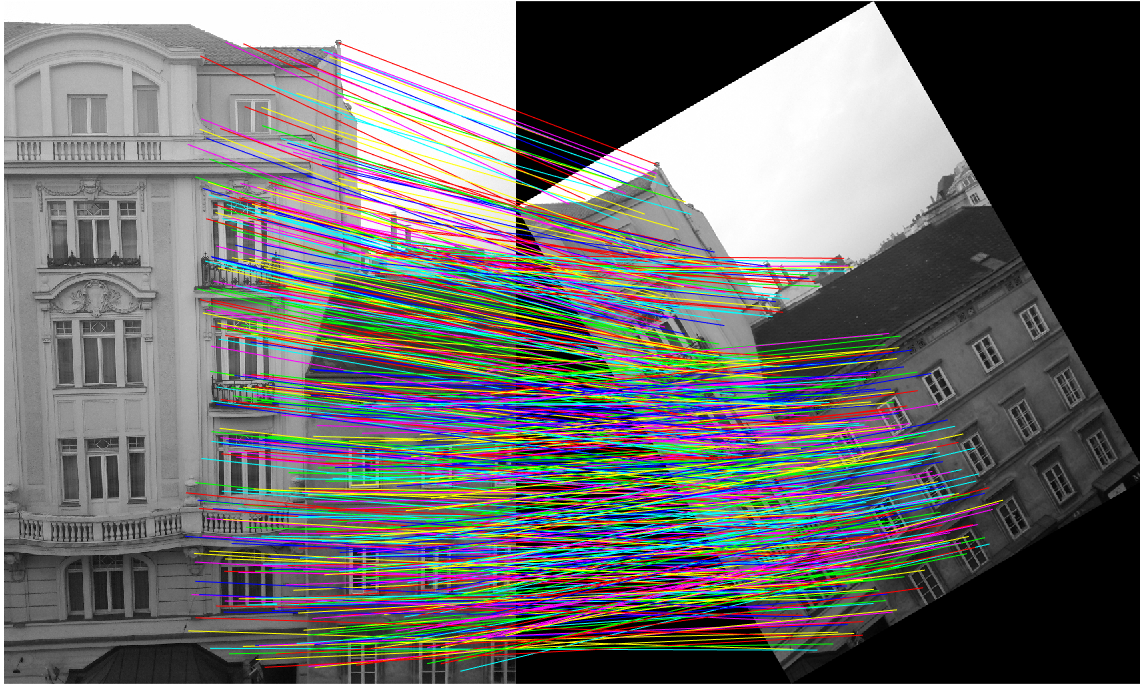
\includegraphics[width=0.59\textwidth]{figures/rotation_ransac.png} &
	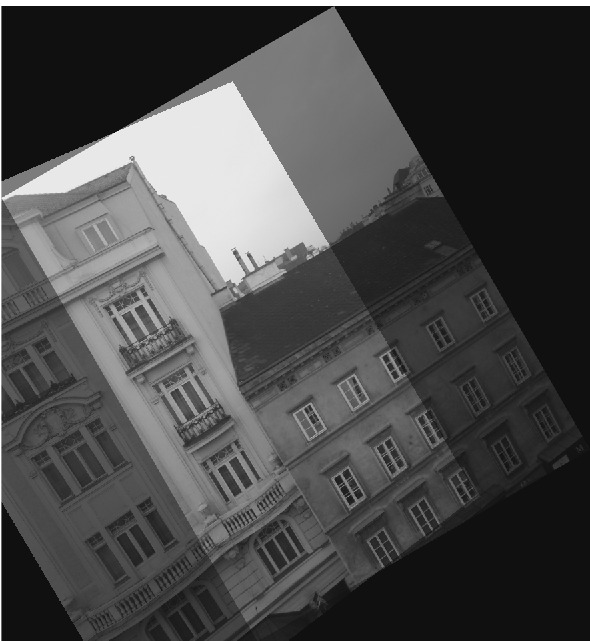
\includegraphics[width=0.33\textwidth]{figures/rotation_overlay.png} 

	\end{tabular}
	\caption{Post RANSAC matches after rotating and rescaling and the aligned result.}
	\label{fig:a4:rotationscale}
\end{figure}

\FloatBarrier % keep figures above!

As described above, the gradient orientation of each pixel is reduced by the key point orientation before being added to the associated histogram. Therefor the result should be invariant to changes in image rotation. Additionally the SIFT algorithm is also scale invariant as described in the first section. This can be seen as illustrated by Figure \ref{fig:a4:rotationscale}.

\subsection{Image Stitching}

To stitch images together for the purpose of creating a panorama view, first the homography is estimated between each pair of adjacent images. An image is selected as reference image (one in the middle of panorama) and utilizing the homographies estimated before, the homography of each image to the reference image is also estimated. Finally each image can be projected into its correct place within the panorama. The results can be viewed on figures \ref{fig:a4:pano1} and \ref{fig:a4:pano2}.

\begin{figure}[h]
	\centering
	\begin{tabular}{cc}
	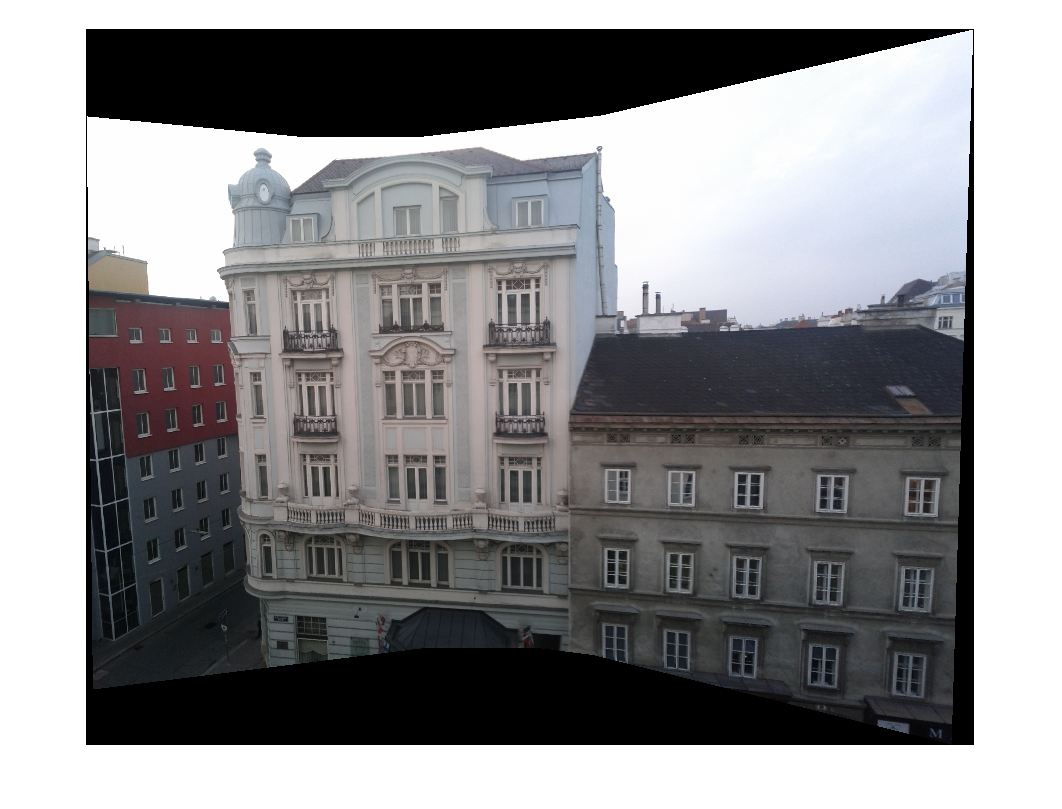
\includegraphics[width=0.8\textwidth]{figures/office_p.png} \\
	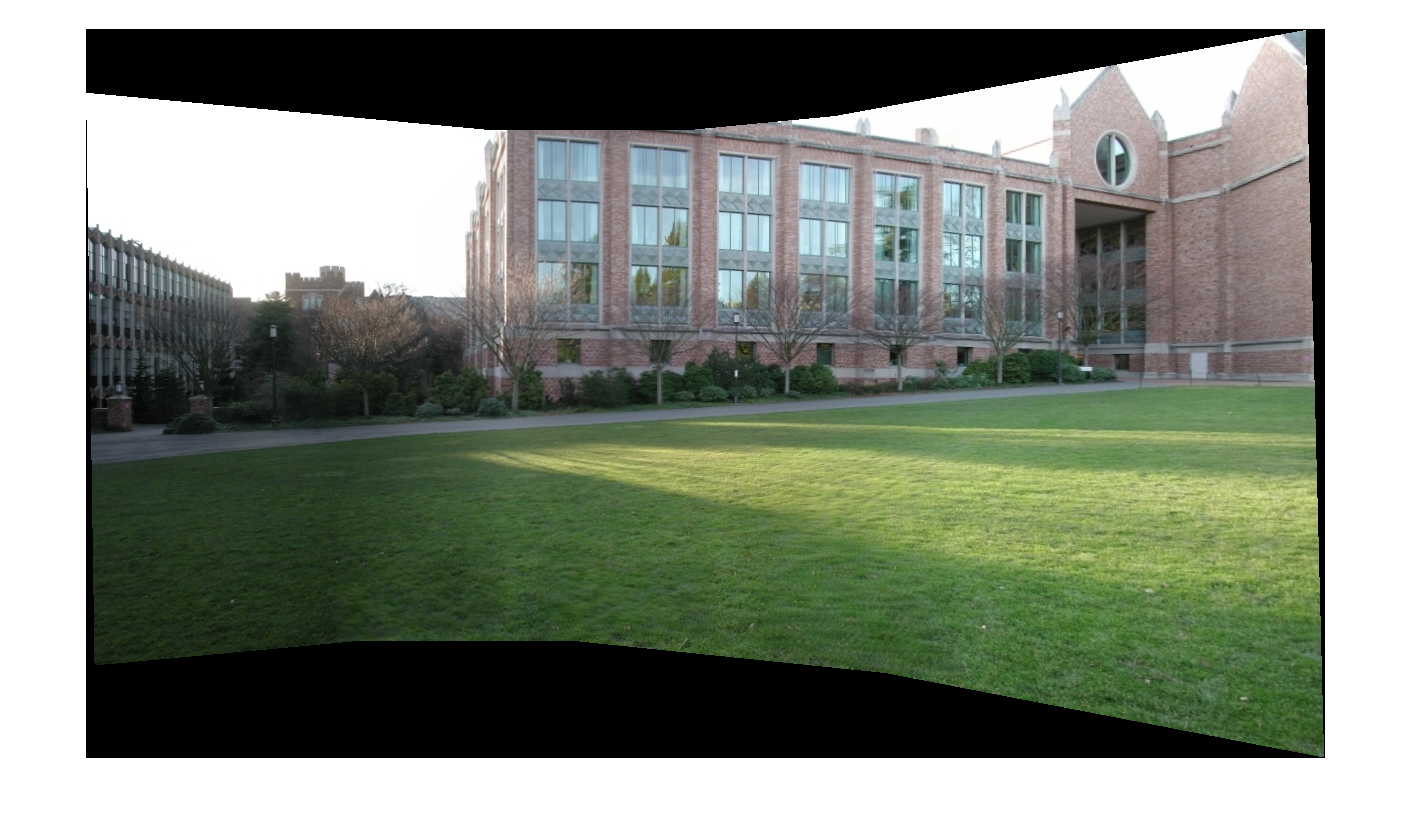
\includegraphics[width=0.8\textwidth]{figures/campus_p.png} 

	\end{tabular}
	\caption{Resulting panorama images with feathering.}
	\label{fig:a4:pano1}
\end{figure}

\begin{figure}[h]
	\centering
	\begin{tabular}{cc}
	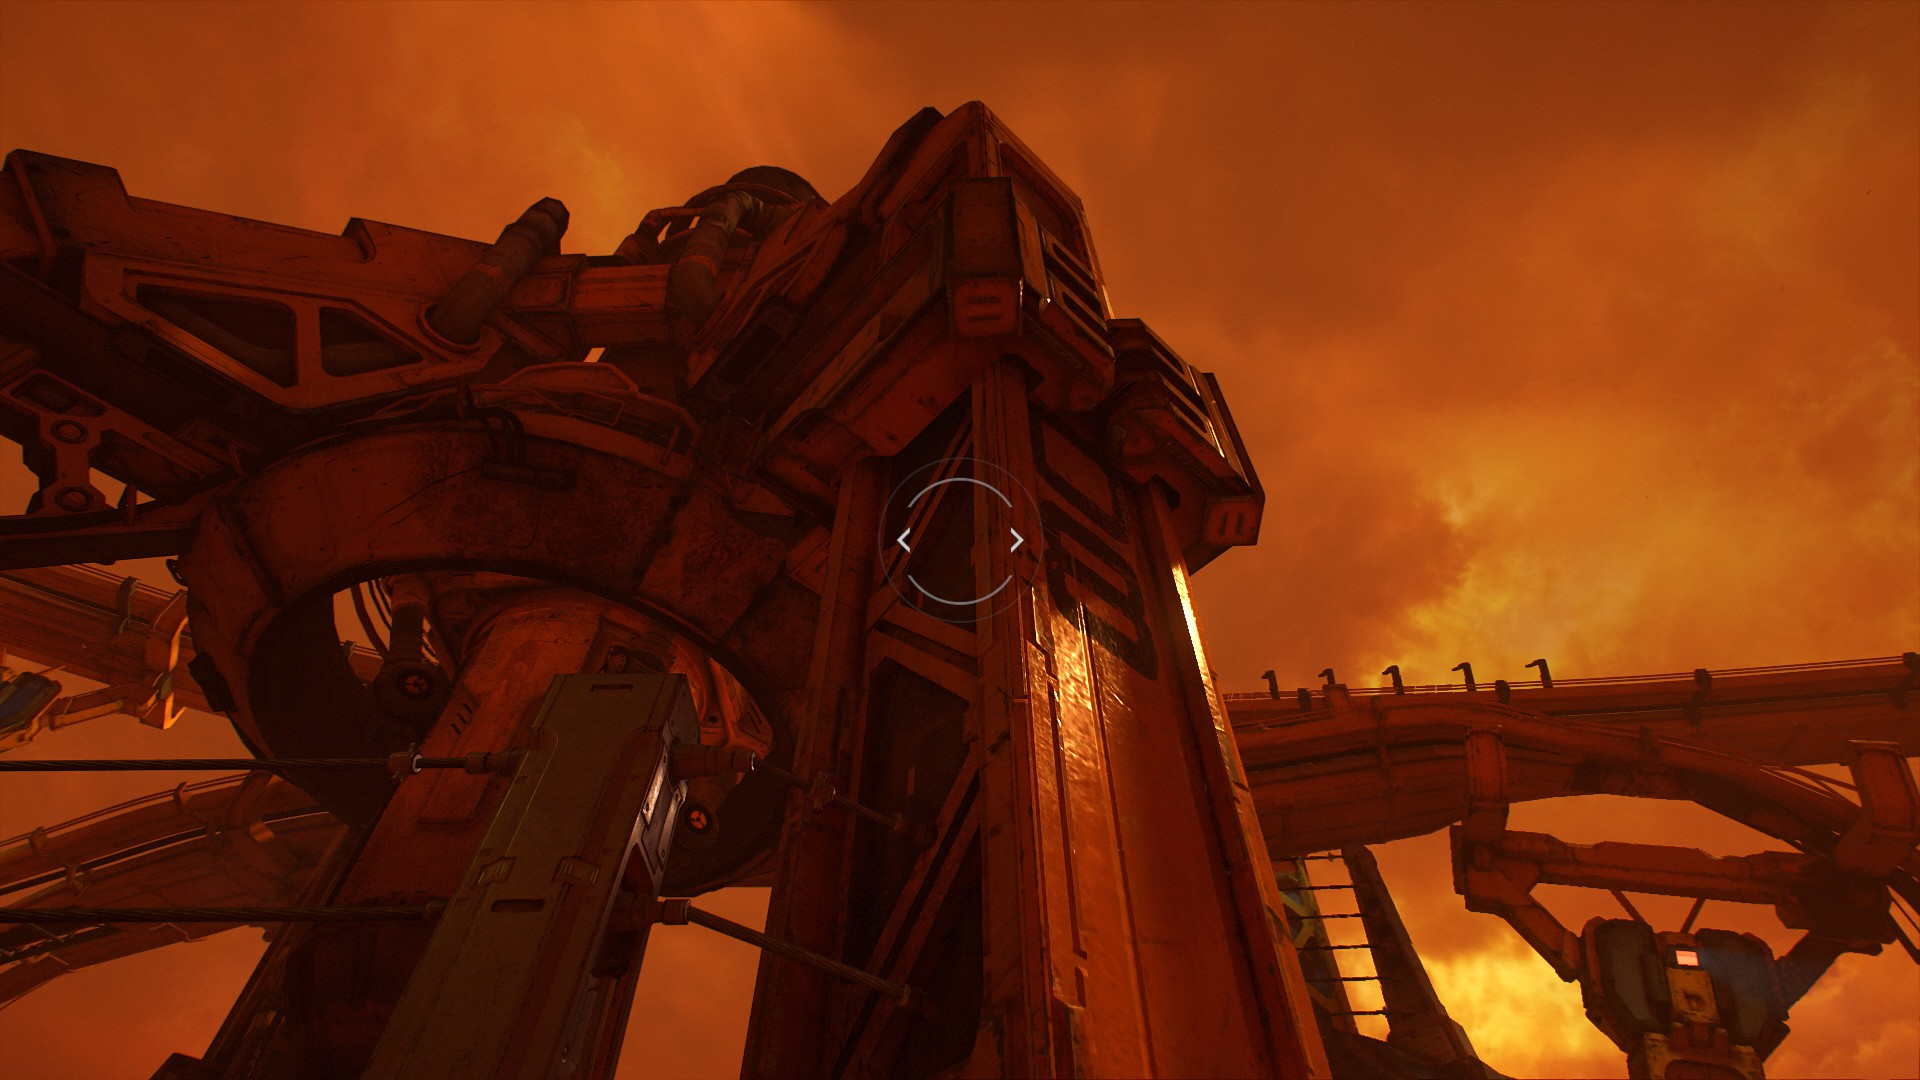
\includegraphics[width=0.33\textwidth]{figures/doom1.jpg}
	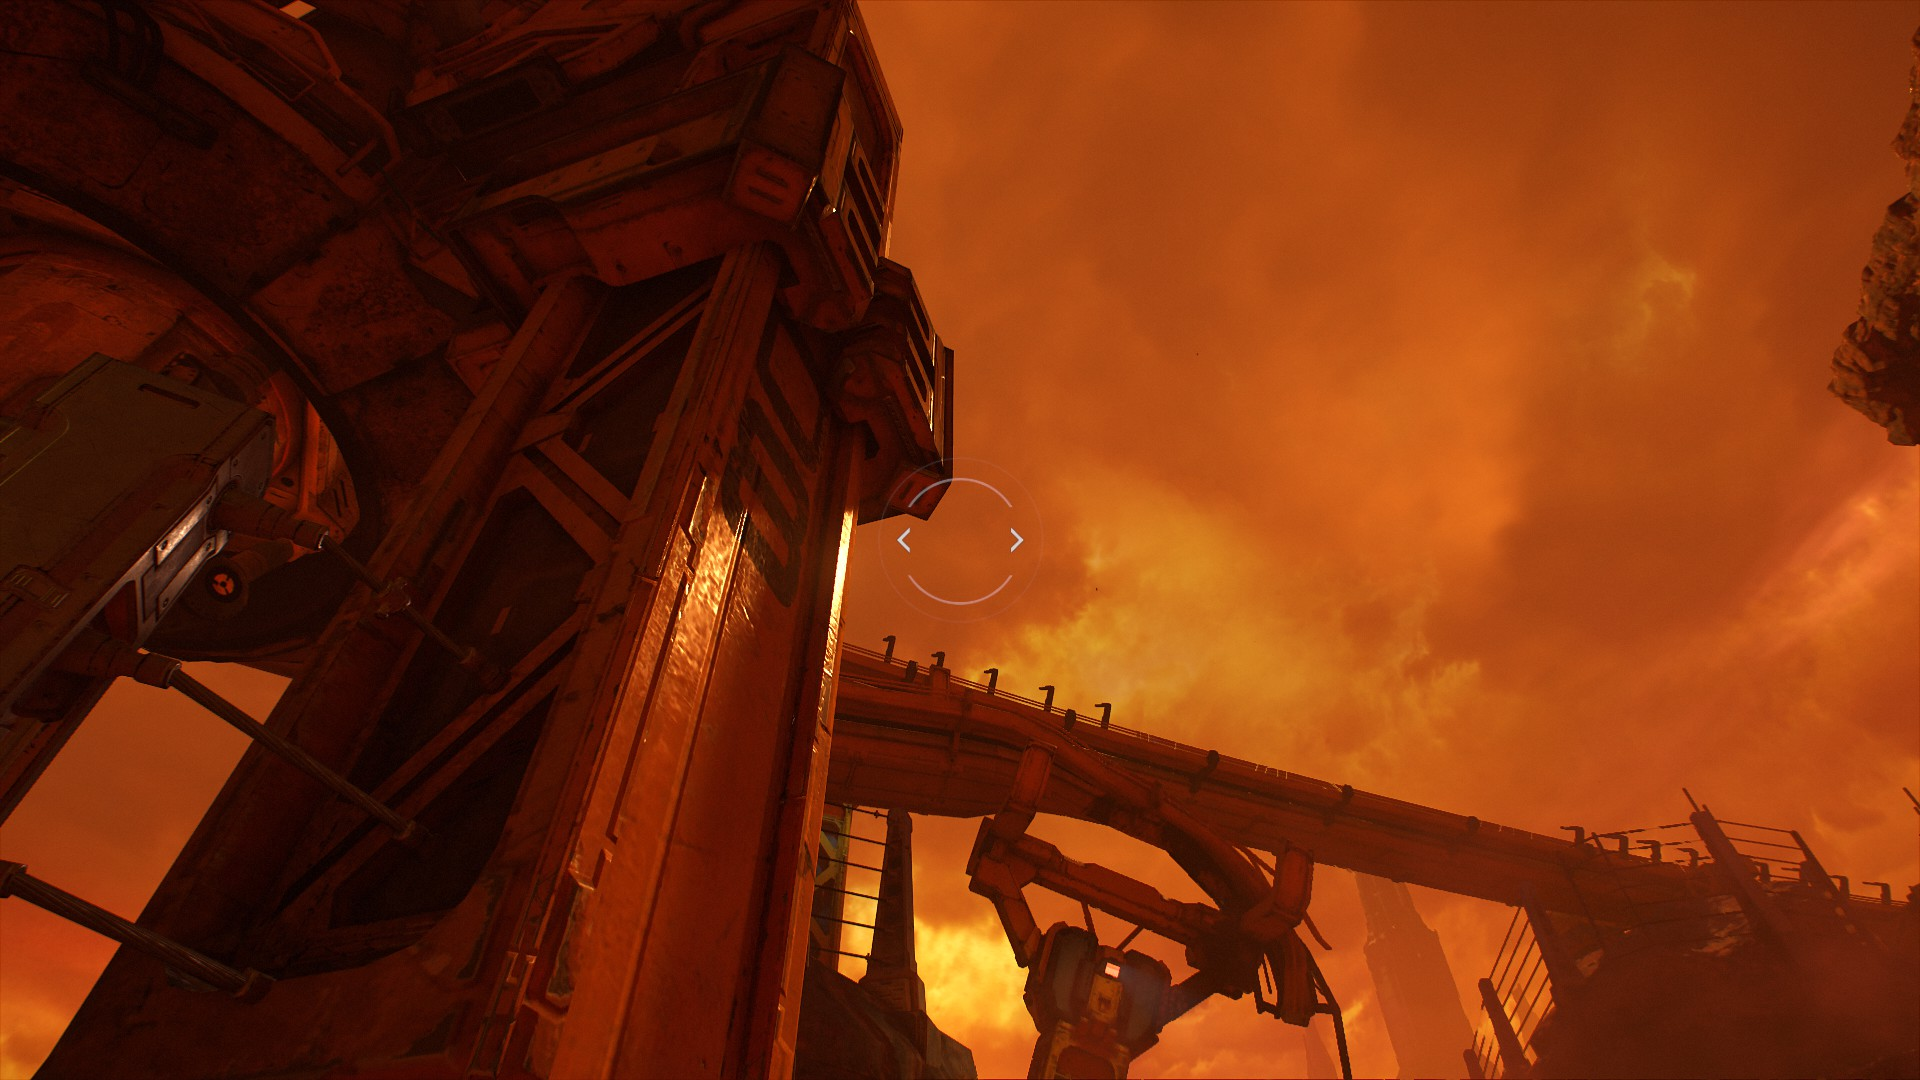
\includegraphics[width=0.33\textwidth]{figures/doom2.jpg}
	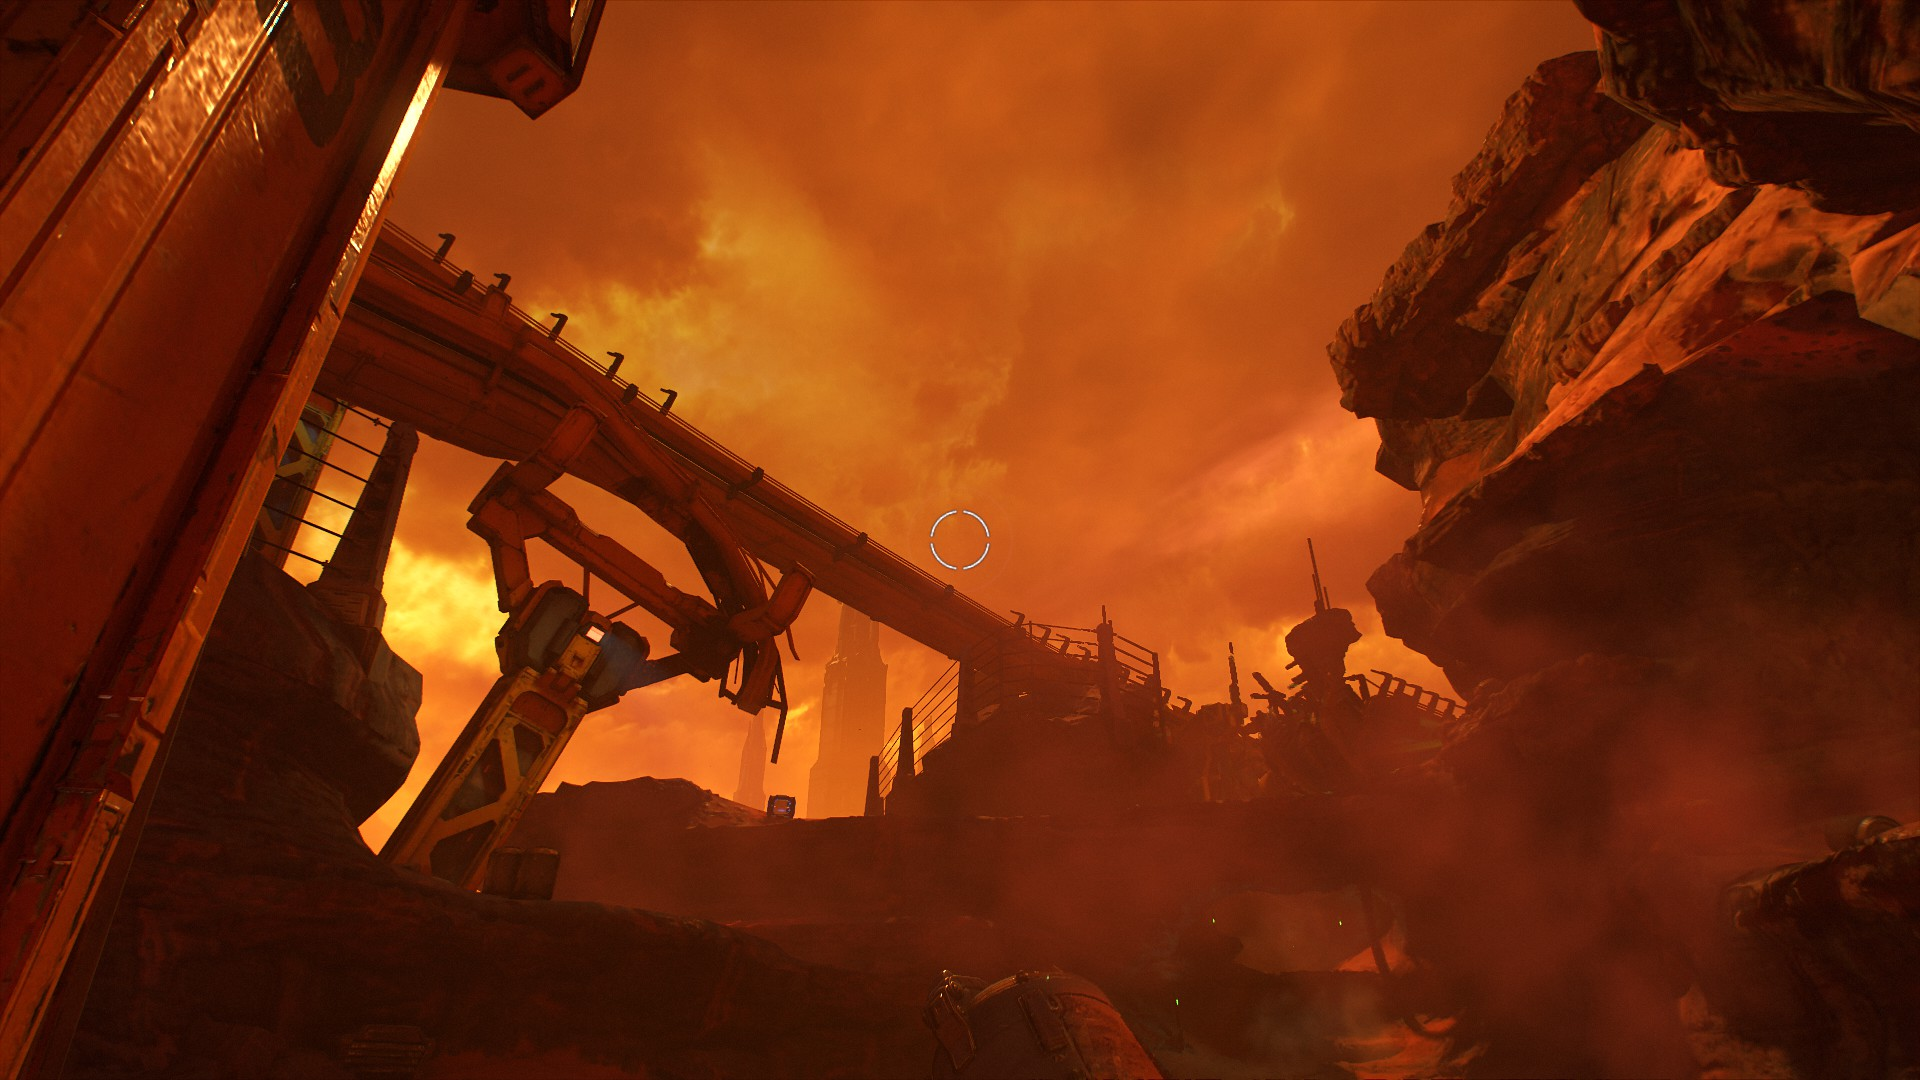
\includegraphics[width=0.33\textwidth]{figures/doom3.jpg} \\
	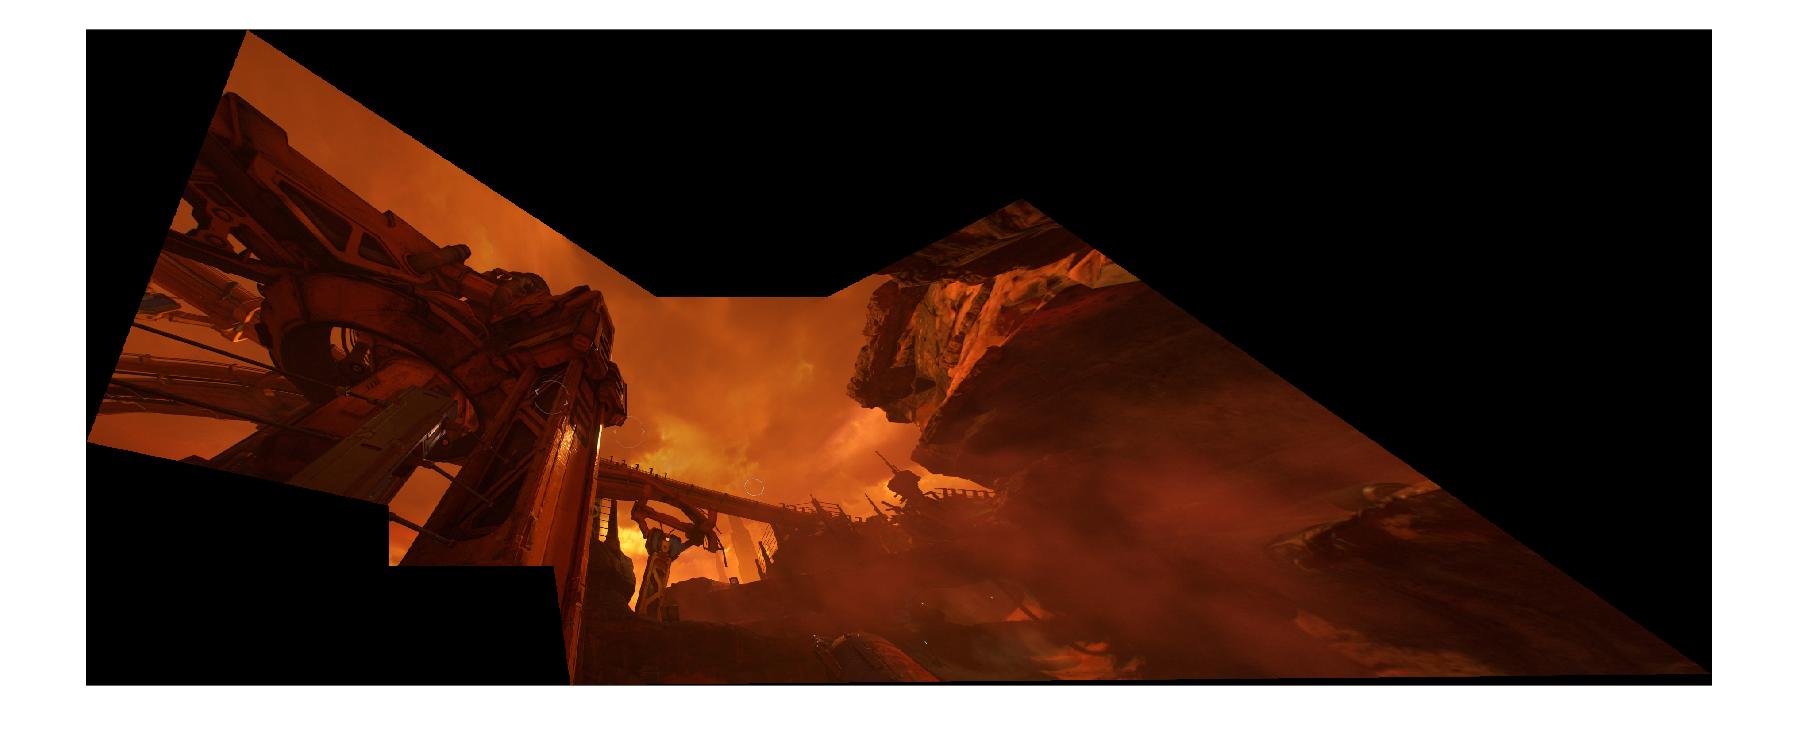
\includegraphics[width=1\textwidth]{figures/doom_p.png}
	
	\end{tabular}
	\caption{Screenshots from the game DOOM (feathering).}
	\label{fig:a4:pano2}
\end{figure}

//note: find and add potential errors here

The panorama images shown in figures \ref{fig:a4:pano1} and \ref{fig:a4:pano2} use feathering to blend the images together. Would we use no blending, the final panorama image would look quite different as illustrated by Figure \ref{fig:a4:noblend}.

\begin{figure}[h]
	\centering
	\begin{tabular}{cc}
	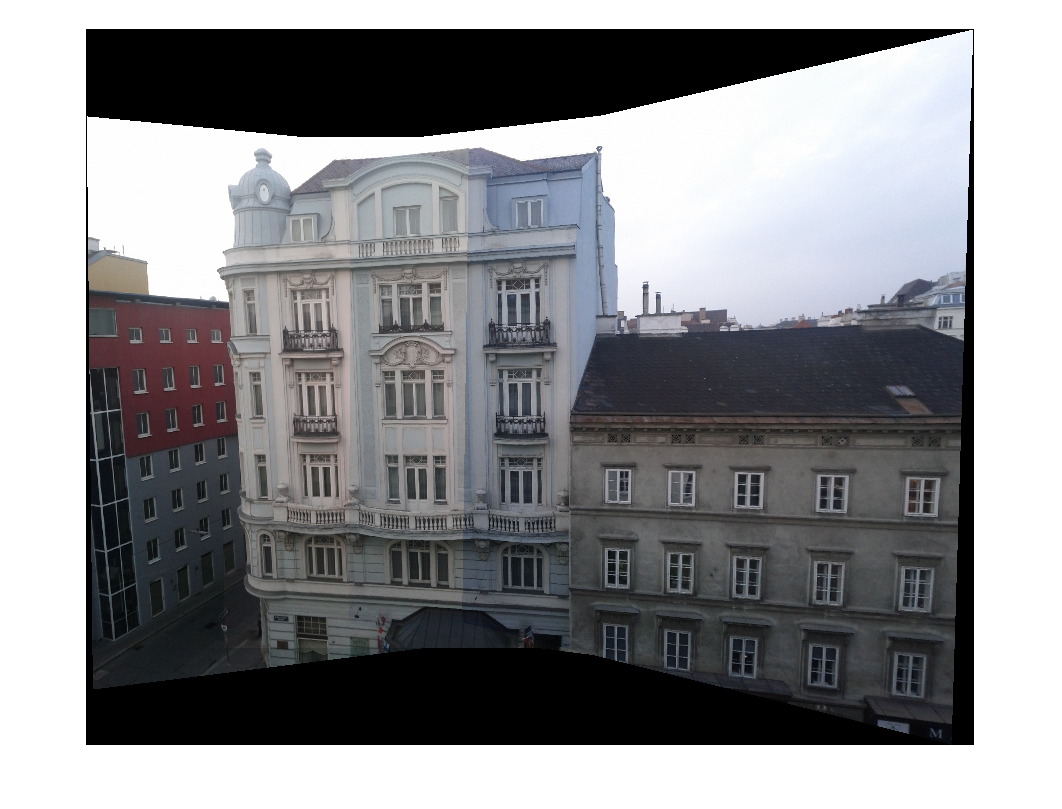
\includegraphics[width=0.8\textwidth]{figures/office_p_b.png} \\
	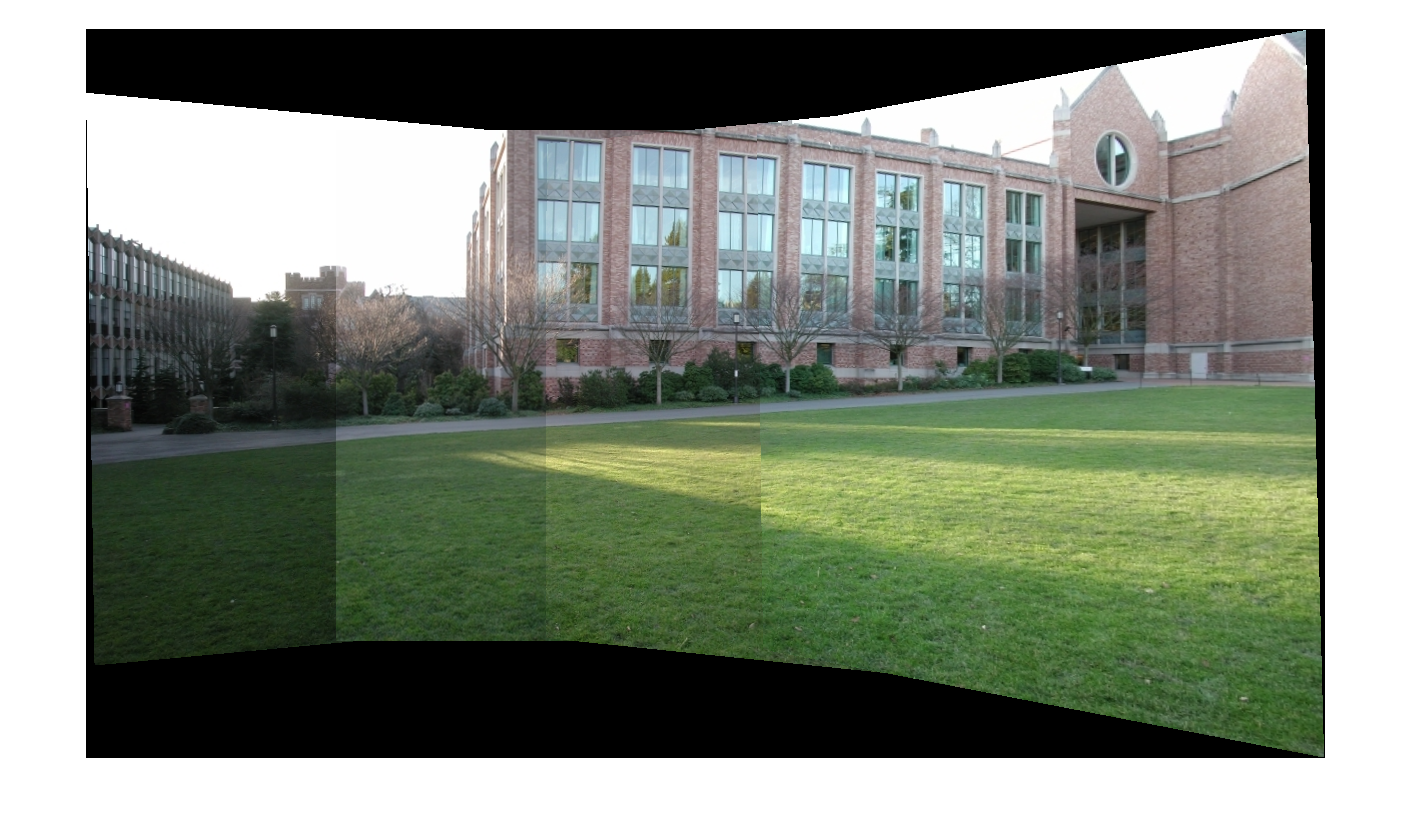
\includegraphics[width=0.8\textwidth]{figures/campus_p_b.png} \\
	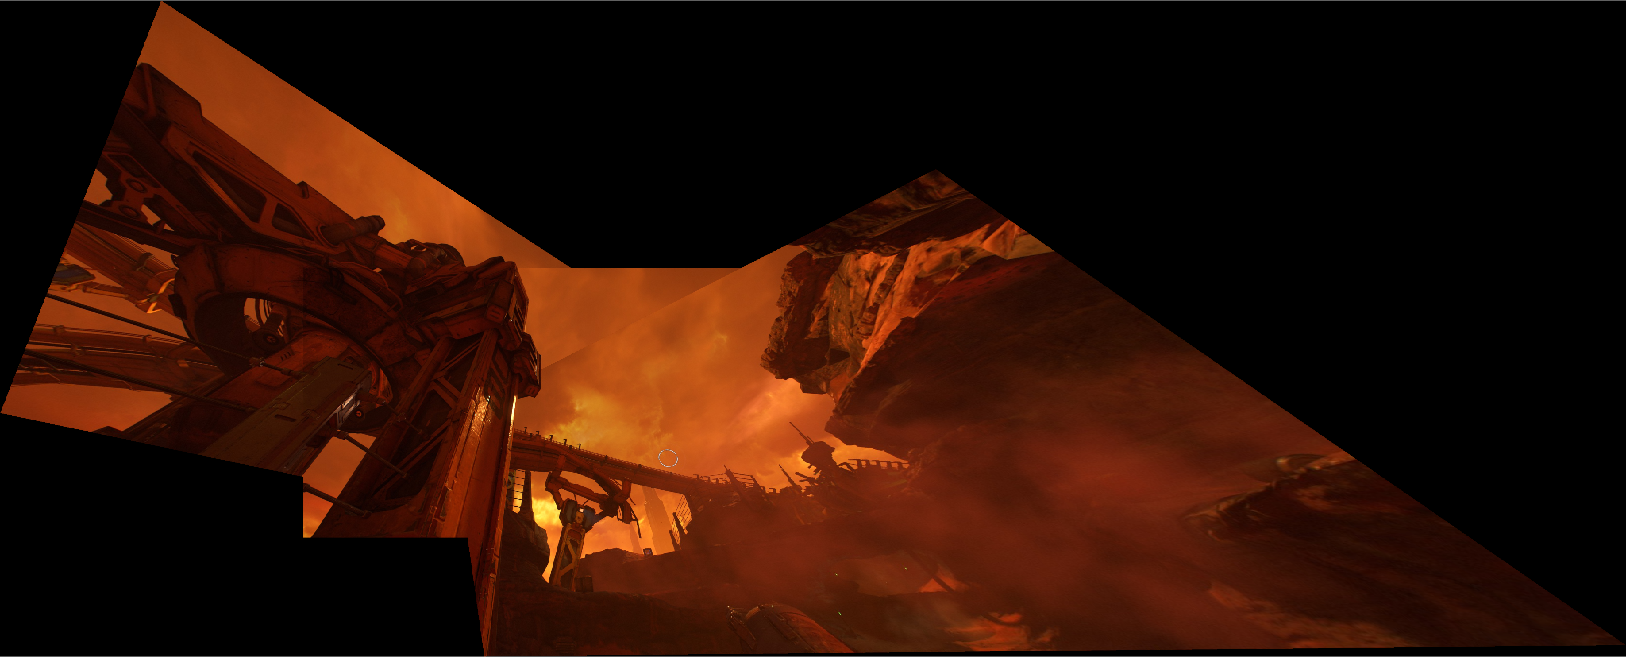
\includegraphics[width=1\textwidth]{figures/doom_p_b.png}

	\end{tabular}
	\caption{Resulting panorama images without blending.}
	\label{fig:a4:noblend}
\end{figure}